\documentclass[twoside]{book}

% Packages required by doxygen
\usepackage{fixltx2e}
\usepackage{calc}
\usepackage{doxygen}
\usepackage[export]{adjustbox} % also loads graphicx
\usepackage{graphicx}
\usepackage[utf8]{inputenc}
\usepackage{makeidx}
\usepackage{multicol}
\usepackage{multirow}
\PassOptionsToPackage{warn}{textcomp}
\usepackage{textcomp}
\usepackage[nointegrals]{wasysym}
\usepackage[table]{xcolor}

% Font selection
\usepackage[T1]{fontenc}
\usepackage[scaled=.90]{helvet}
\usepackage{courier}
\usepackage{amssymb}
\usepackage{sectsty}
\renewcommand{\familydefault}{\sfdefault}
\allsectionsfont{%
  \fontseries{bc}\selectfont%
  \color{darkgray}%
}
\renewcommand{\DoxyLabelFont}{%
  \fontseries{bc}\selectfont%
  \color{darkgray}%
}
\newcommand{\+}{\discretionary{\mbox{\scriptsize$\hookleftarrow$}}{}{}}

% Page & text layout
\usepackage{geometry}
\geometry{%
  a4paper,%
  top=2.5cm,%
  bottom=2.5cm,%
  left=2.5cm,%
  right=2.5cm%
}
\tolerance=750
\hfuzz=15pt
\hbadness=750
\setlength{\emergencystretch}{15pt}
\setlength{\parindent}{0cm}
\setlength{\parskip}{3ex plus 2ex minus 2ex}
\makeatletter
\renewcommand{\paragraph}{%
  \@startsection{paragraph}{4}{0ex}{-1.0ex}{1.0ex}{%
    \normalfont\normalsize\bfseries\SS@parafont%
  }%
}
\renewcommand{\subparagraph}{%
  \@startsection{subparagraph}{5}{0ex}{-1.0ex}{1.0ex}{%
    \normalfont\normalsize\bfseries\SS@subparafont%
  }%
}
\makeatother

% Headers & footers
\usepackage{fancyhdr}
\pagestyle{fancyplain}
\fancyhead[LE]{\fancyplain{}{\bfseries\thepage}}
\fancyhead[CE]{\fancyplain{}{}}
\fancyhead[RE]{\fancyplain{}{\bfseries\leftmark}}
\fancyhead[LO]{\fancyplain{}{\bfseries\rightmark}}
\fancyhead[CO]{\fancyplain{}{}}
\fancyhead[RO]{\fancyplain{}{\bfseries\thepage}}
\fancyfoot[LE]{\fancyplain{}{}}
\fancyfoot[CE]{\fancyplain{}{}}
\fancyfoot[RE]{\fancyplain{}{\bfseries\scriptsize Generated by Doxygen }}
\fancyfoot[LO]{\fancyplain{}{\bfseries\scriptsize Generated by Doxygen }}
\fancyfoot[CO]{\fancyplain{}{}}
\fancyfoot[RO]{\fancyplain{}{}}
\renewcommand{\footrulewidth}{0.4pt}
\renewcommand{\chaptermark}[1]{%
  \markboth{#1}{}%
}
\renewcommand{\sectionmark}[1]{%
  \markright{\thesection\ #1}%
}

% Indices & bibliography
\usepackage{natbib}
\usepackage[titles]{tocloft}
\setcounter{tocdepth}{3}
\setcounter{secnumdepth}{5}
\makeindex

% Hyperlinks (required, but should be loaded last)
\usepackage{ifpdf}
\ifpdf
  \usepackage[pdftex,pagebackref=true]{hyperref}
\else
  \usepackage[ps2pdf,pagebackref=true]{hyperref}
\fi
\hypersetup{%
  colorlinks=true,%
  linkcolor=blue,%
  citecolor=blue,%
  unicode%
}

% Custom commands
\newcommand{\clearemptydoublepage}{%
  \newpage{\pagestyle{empty}\cleardoublepage}%
}

\usepackage{caption}
\captionsetup{labelsep=space,justification=centering,font={bf},singlelinecheck=off,skip=4pt,position=top}

%===== C O N T E N T S =====

\begin{document}

% Titlepage & ToC
\hypersetup{pageanchor=false,
             bookmarksnumbered=true,
             pdfencoding=unicode
            }
\pagenumbering{alph}
\begin{titlepage}
\vspace*{7cm}
\begin{center}%
{\Large Lidar filters }\\
\vspace*{1cm}
{\large Generated by Doxygen 1.8.13}\\
\end{center}
\end{titlepage}
\clearemptydoublepage
\pagenumbering{roman}
\tableofcontents
\clearemptydoublepage
\pagenumbering{arabic}
\hypersetup{pageanchor=true}

%--- Begin generated contents ---
\chapter{Main Page}
\label{index}\hypertarget{index}{}\hypertarget{index_build_test_sec}{}\section{Build and run unit tests}\label{index_build_test_sec}
In order to build the code you will need g++, make and pthread. To make and run the tests do \+:

\$$>$ make test

There are two tests in the suite, one for the Range flter and one for the Temporal median filter. Both should show \textquotesingle{}P\+A\+S\+S\+ED\textquotesingle{} if successful or \textquotesingle{}F\+A\+I\+L\+ED\textquotesingle{} on error.\hypertarget{index_build_docs_sec}{}\section{Build this documentation}\label{index_build_docs_sec}
If you have Doxygen installed you can rebuild this documentartion with

\$$>$ make docs

The documentation main page is at docs/html/index.\+html\hypertarget{index_usage_sec}{}\section{Using the filters}\label{index_usage_sec}
\hypertarget{index_rangeFilter}{}\subsection{\+: Range\+Filter}\label{index_rangeFilter}
Example usage \+: 
\begin{DoxyCodeInclude}
    
    \textcolor{comment}{// Create range filter object}
    \hyperlink{class_range_filter}{RangeFilter} rf(0.03, 50.0); \textcolor{comment}{// Or if using default contructor the min and max are assumed}
    
    \textcolor{keywordtype}{float} inArr0[] = \{-10.0, 0.029, 0.03, 10.0, 20.0, 30.0, 40.0, 50.0, 50.1, 60.0\};
    \textcolor{keywordtype}{float} outArr0[] = \{0.03, 0.03, 0.03, 10.0, 20.0, 30.0, 40.0, 50.0, 50.0, 50.0\}; \textcolor{comment}{// expected output}
    
    std::vector<float> inVec0 (inArr0, inArr0 + \textcolor{keyword}{sizeof}(inArr0) / \textcolor{keyword}{sizeof}(inArr0[0]) );
    std::vector<float> outVec0 (outArr0, outArr0 + \textcolor{keyword}{sizeof}(outArr0) / \textcolor{keyword}{sizeof}(outArr0[0]) );
    
    rf.update(inVec0);
    
    \textcolor{keywordflow}{if}(!(inVec0 == outVec0)) \{
        \textcolor{comment}{// Report error for this test and continue}
        std::cout << \textcolor{stringliteral}{"Range filter returned unexpected output "} << std::endl;
        std::cout << \textcolor{stringliteral}{"\(\backslash\)nExpected array : "};
        printVec(outVec0);
        
        std::cout << \textcolor{stringliteral}{"\(\backslash\)nReturned array : "};
        printVec(inVec0);
        std::cout << std::endl;
        
        \textcolor{keywordflow}{throw}(-1);
    \}
\end{DoxyCodeInclude}
 \hypertarget{index_temporalFilter}{}\subsection{\+: Temporal\+Filter}\label{index_temporalFilter}
Example usage \+: 
\begin{DoxyCodeInclude}
    \textcolor{comment}{// create filter object}
    \hyperlink{class_temporal_filter}{TemporalFilter} tf(3); \textcolor{comment}{// Depth set to 3}
    
    \textcolor{comment}{// scanline 1}
    \textcolor{keywordtype}{float} inArr0[] = \{0.0, 1.0, 2.0, 1.0, 3.0 \};  \textcolor{comment}{// input scanline}
    \textcolor{keywordtype}{float} outArr0[] = \{0.0, 1.0, 2.0, 1.0, 3.0 \}; \textcolor{comment}{// expected output}
    
    std::vector<float> inVec0 (inArr0, inArr0 + \textcolor{keyword}{sizeof}(inArr0) / \textcolor{keyword}{sizeof}(inArr0[0]) );
    std::vector<float> outVec0 (outArr0, outArr0 + \textcolor{keyword}{sizeof}(outArr0) / \textcolor{keyword}{sizeof}(outArr0[0]) );
    
    tf.update(inVec0);
    
    \textcolor{keywordflow}{if}(!(inVec0 == outVec0)) \{
        std::cout << \textcolor{stringliteral}{"\(\backslash\)nExpected : "}; printVec(outVec0);
        std::cout << \textcolor{stringliteral}{"\(\backslash\)nReceived : "}; printVec(inVec0);
        
        \textcolor{keywordflow}{throw}(-1);
    \}
    
\end{DoxyCodeInclude}

\chapter{Hierarchical Index}
\section{Class Hierarchy}
This inheritance list is sorted roughly, but not completely, alphabetically\+:\begin{DoxyCompactList}
\item \contentsline{section}{Filter}{\pageref{class_filter}}{}
\begin{DoxyCompactList}
\item \contentsline{section}{Range\+Filter}{\pageref{class_range_filter}}{}
\item \contentsline{section}{Temporal\+Filter}{\pageref{class_temporal_filter}}{}
\end{DoxyCompactList}
\item \contentsline{section}{median\+Thread\+Params}{\pageref{structmedian_thread_params}}{}
\end{DoxyCompactList}

\chapter{Class Index}
\section{Class List}
Here are the classes, structs, unions and interfaces with brief descriptions\+:\begin{DoxyCompactList}
\item\contentsline{section}{\hyperlink{class_filter}{Filter} \\*Abstract class used as a base class for the range and temporal median filters }{\pageref{class_filter}}{}
\item\contentsline{section}{\hyperlink{structmedian_thread_params}{median\+Thread\+Params} \\*Struct passed as arguments to the compute threads for temporal median filter }{\pageref{structmedian_thread_params}}{}
\item\contentsline{section}{\hyperlink{class_range_filter}{Range\+Filter} \\*Range filter class }{\pageref{class_range_filter}}{}
\item\contentsline{section}{\hyperlink{class_temporal_filter}{Temporal\+Filter} \\*Temporal Median filter class }{\pageref{class_temporal_filter}}{}
\end{DoxyCompactList}

\chapter{Class Documentation}
\hypertarget{class_filter}{}\section{Filter Class Reference}
\label{class_filter}\index{Filter@{Filter}}


Abstract class used as a base class for the range and temporal median filters.  




{\ttfamily \#include $<$filter.\+hpp$>$}

Inheritance diagram for Filter\+:\begin{figure}[H]
\begin{center}
\leavevmode
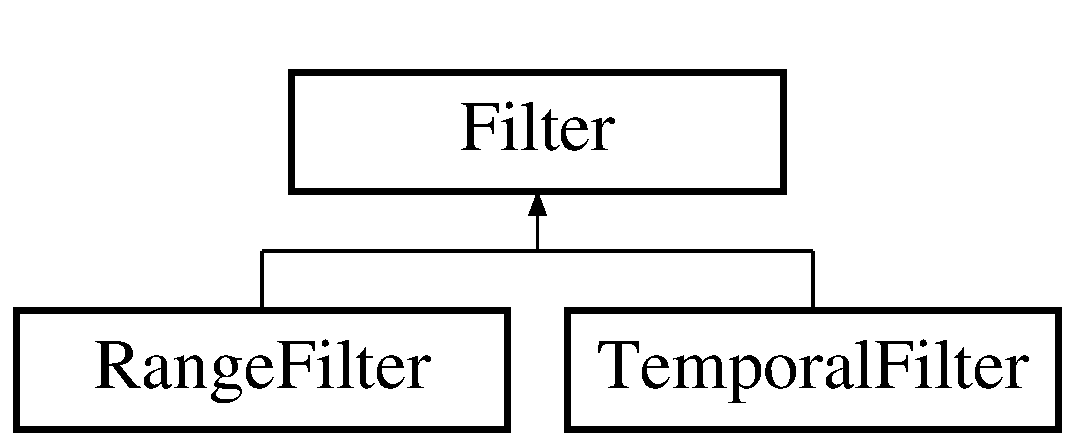
\includegraphics[height=2.000000cm]{class_filter}
\end{center}
\end{figure}
\subsection*{Public Member Functions}
\begin{DoxyCompactItemize}
\item 
\mbox{\Hypertarget{class_filter_a3a4cfdec9a607efe139b7648dfda0caf}\label{class_filter_a3a4cfdec9a607efe139b7648dfda0caf}} 
virtual std\+::vector$<$ float $>$ {\bfseries update} (std\+::vector$<$ float $>$ \&)=0
\item 
void \hyperlink{class_filter_a68763fa259eb46616b104d7342d727f1}{filter} ()
\end{DoxyCompactItemize}


\subsection{Detailed Description}
Abstract class used as a base class for the range and temporal median filters. 

\begin{DoxyAuthor}{Author}
Raj Singh (\href{mailto:rajvikrams@gmail.com}{\tt rajvikrams@gmail.\+com}) 
\end{DoxyAuthor}
\begin{DoxyVersion}{Version}
0.\+1 
\end{DoxyVersion}
\begin{DoxyDate}{Date}
09-\/11-\/2017
\end{DoxyDate}
Child classes will have to implement the update() method. 

\subsection{Member Function Documentation}
\mbox{\Hypertarget{class_filter_a68763fa259eb46616b104d7342d727f1}\label{class_filter_a68763fa259eb46616b104d7342d727f1}} 
\index{Filter@{Filter}!filter@{filter}}
\index{filter@{filter}!Filter@{Filter}}
\subsubsection{\texorpdfstring{filter()}{filter()}}
{\footnotesize\ttfamily void Filter\+::filter (\begin{DoxyParamCaption}{ }\end{DoxyParamCaption})\hspace{0.3cm}{\ttfamily [inline]}}

Pure virtual update method 

The documentation for this class was generated from the following file\+:\begin{DoxyCompactItemize}
\item 
filter.\+hpp\end{DoxyCompactItemize}

\hypertarget{structmedian_thread_params}{}\section{median\+Thread\+Params Struct Reference}
\label{structmedian_thread_params}\index{median\+Thread\+Params@{median\+Thread\+Params}}


Struct passed as arguments to the compute threads for temporal median filter.  




{\ttfamily \#include $<$temporal\+Filter.\+hpp$>$}

\subsection*{Public Attributes}
\begin{DoxyCompactItemize}
\item 
\mbox{\Hypertarget{structmedian_thread_params_a8db108c4609858e869578e9765954486}\label{structmedian_thread_params_a8db108c4609858e869578e9765954486}} 
int {\bfseries my\+Id}
\item 
\mbox{\Hypertarget{structmedian_thread_params_ab5a693b517ff20c278208aa3b2a20b54}\label{structmedian_thread_params_ab5a693b517ff20c278208aa3b2a20b54}} 
int {\bfseries thread\+Pool\+Count}
\item 
\mbox{\Hypertarget{structmedian_thread_params_a4bac74b30318ffb7d08cb358215319db}\label{structmedian_thread_params_a4bac74b30318ffb7d08cb358215319db}} 
std\+::vector$<$ std\+::vector$<$ float $>$ $>$ $\ast$ {\bfseries input\+Scanlines}
\item 
\mbox{\Hypertarget{structmedian_thread_params_ae615afd49e1de11d8471bc27b48df7ae}\label{structmedian_thread_params_ae615afd49e1de11d8471bc27b48df7ae}} 
std\+::vector$<$ float $>$ $\ast$ {\bfseries output\+Scanline}
\end{DoxyCompactItemize}


\subsection{Detailed Description}
Struct passed as arguments to the compute threads for temporal median filter. 

\begin{DoxyAuthor}{Author}
Raj Singh (\href{mailto:rajvikrams@gmail.com}{\tt rajvikrams@gmail.\+com}) 
\end{DoxyAuthor}
\begin{DoxyVersion}{Version}
0.\+1 
\end{DoxyVersion}
\begin{DoxyDate}{Date}
09-\/11-\/2017 
\end{DoxyDate}


The documentation for this struct was generated from the following file\+:\begin{DoxyCompactItemize}
\item 
temporal\+Filter.\+hpp\end{DoxyCompactItemize}

\hypertarget{class_range_filter}{}\section{Range\+Filter Class Reference}
\label{class_range_filter}\index{Range\+Filter@{Range\+Filter}}


Range filter class.  




{\ttfamily \#include $<$range\+Filter.\+hpp$>$}

Inheritance diagram for Range\+Filter\+:\begin{figure}[H]
\begin{center}
\leavevmode
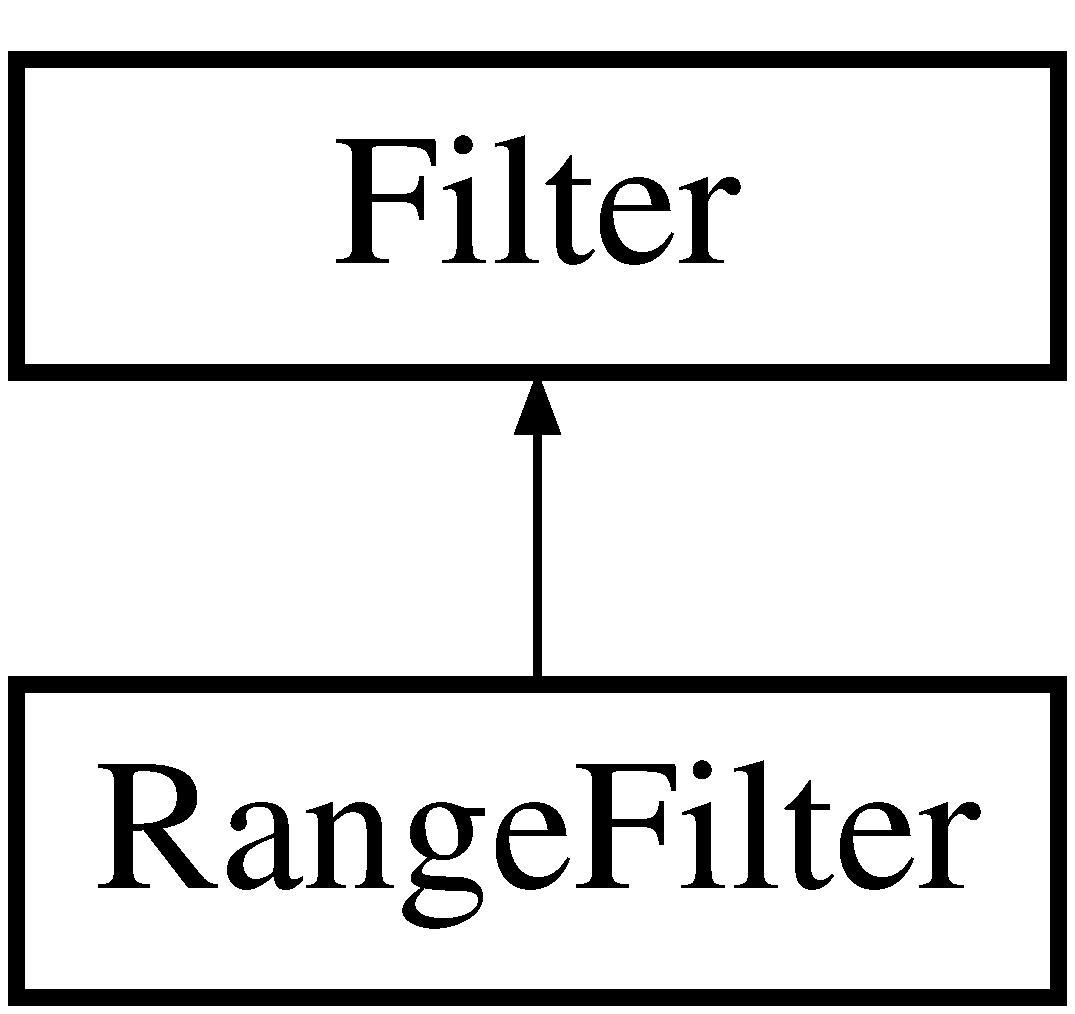
\includegraphics[height=2.000000cm]{class_range_filter}
\end{center}
\end{figure}
\subsection*{Public Member Functions}
\begin{DoxyCompactItemize}
\item 
\hyperlink{class_range_filter_ad0b28929ddfb283eb0101b00726d1729}{Range\+Filter} ()
\item 
\hyperlink{class_range_filter_afed8c9dea5d2c7857075bfd1f64648a4}{Range\+Filter} (float min, float max)
\item 
std\+::vector$<$ float $>$ \hyperlink{class_range_filter_a6160f4ffe6788fb7fe935110ad941568}{update} (std\+::vector$<$ float $>$ \&scan\+Line)
\end{DoxyCompactItemize}


\subsection{Detailed Description}
Range filter class. 

\begin{DoxyAuthor}{Author}
Raj Singh (\href{mailto:rajvikrams@gmail.com}{\tt rajvikrams@gmail.\+com}) 
\end{DoxyAuthor}
\begin{DoxyVersion}{Version}
0.\+1 
\end{DoxyVersion}
\begin{DoxyDate}{Date}
09-\/11-\/2017
\end{DoxyDate}
Implements an update method that clamps scanline values to min and max specified by the constructor. 

\subsection{Constructor \& Destructor Documentation}
\mbox{\Hypertarget{class_range_filter_ad0b28929ddfb283eb0101b00726d1729}\label{class_range_filter_ad0b28929ddfb283eb0101b00726d1729}} 
\index{Range\+Filter@{Range\+Filter}!Range\+Filter@{Range\+Filter}}
\index{Range\+Filter@{Range\+Filter}!Range\+Filter@{Range\+Filter}}
\subsubsection{\texorpdfstring{Range\+Filter()}{RangeFilter()}\hspace{0.1cm}{\footnotesize\ttfamily [1/2]}}
{\footnotesize\ttfamily Range\+Filter\+::\+Range\+Filter (\begin{DoxyParamCaption}{ }\end{DoxyParamCaption})\hspace{0.3cm}{\ttfamily [inline]}}

Default constructor dist\+Min defaults to 0.\+03

dist\+Max defaults to 50.\+0 \mbox{\Hypertarget{class_range_filter_afed8c9dea5d2c7857075bfd1f64648a4}\label{class_range_filter_afed8c9dea5d2c7857075bfd1f64648a4}} 
\index{Range\+Filter@{Range\+Filter}!Range\+Filter@{Range\+Filter}}
\index{Range\+Filter@{Range\+Filter}!Range\+Filter@{Range\+Filter}}
\subsubsection{\texorpdfstring{Range\+Filter()}{RangeFilter()}\hspace{0.1cm}{\footnotesize\ttfamily [2/2]}}
{\footnotesize\ttfamily Range\+Filter\+::\+Range\+Filter (\begin{DoxyParamCaption}\item[{float}]{min,  }\item[{float}]{max }\end{DoxyParamCaption})\hspace{0.3cm}{\ttfamily [inline]}}

Constructor with min and max 

\subsection{Member Function Documentation}
\mbox{\Hypertarget{class_range_filter_a6160f4ffe6788fb7fe935110ad941568}\label{class_range_filter_a6160f4ffe6788fb7fe935110ad941568}} 
\index{Range\+Filter@{Range\+Filter}!update@{update}}
\index{update@{update}!Range\+Filter@{Range\+Filter}}
\subsubsection{\texorpdfstring{update()}{update()}}
{\footnotesize\ttfamily std\+::vector$<$float$>$ Range\+Filter\+::update (\begin{DoxyParamCaption}\item[{std\+::vector$<$ float $>$ \&}]{scan\+Line }\end{DoxyParamCaption})\hspace{0.3cm}{\ttfamily [inline]}, {\ttfamily [virtual]}}

Method takes in a scanline vector object and clamps the object\textquotesingle{}s values between min and max. Returns the modified object upon success 

Implements \hyperlink{class_filter}{Filter}.



The documentation for this class was generated from the following file\+:\begin{DoxyCompactItemize}
\item 
range\+Filter.\+hpp\end{DoxyCompactItemize}

\hypertarget{class_temporal_filter}{}\section{Temporal\+Filter Class Reference}
\label{class_temporal_filter}\index{Temporal\+Filter@{Temporal\+Filter}}


Temporal Median filter class.  




{\ttfamily \#include $<$temporal\+Filter.\+hpp$>$}

Inheritance diagram for Temporal\+Filter\+:\begin{figure}[H]
\begin{center}
\leavevmode
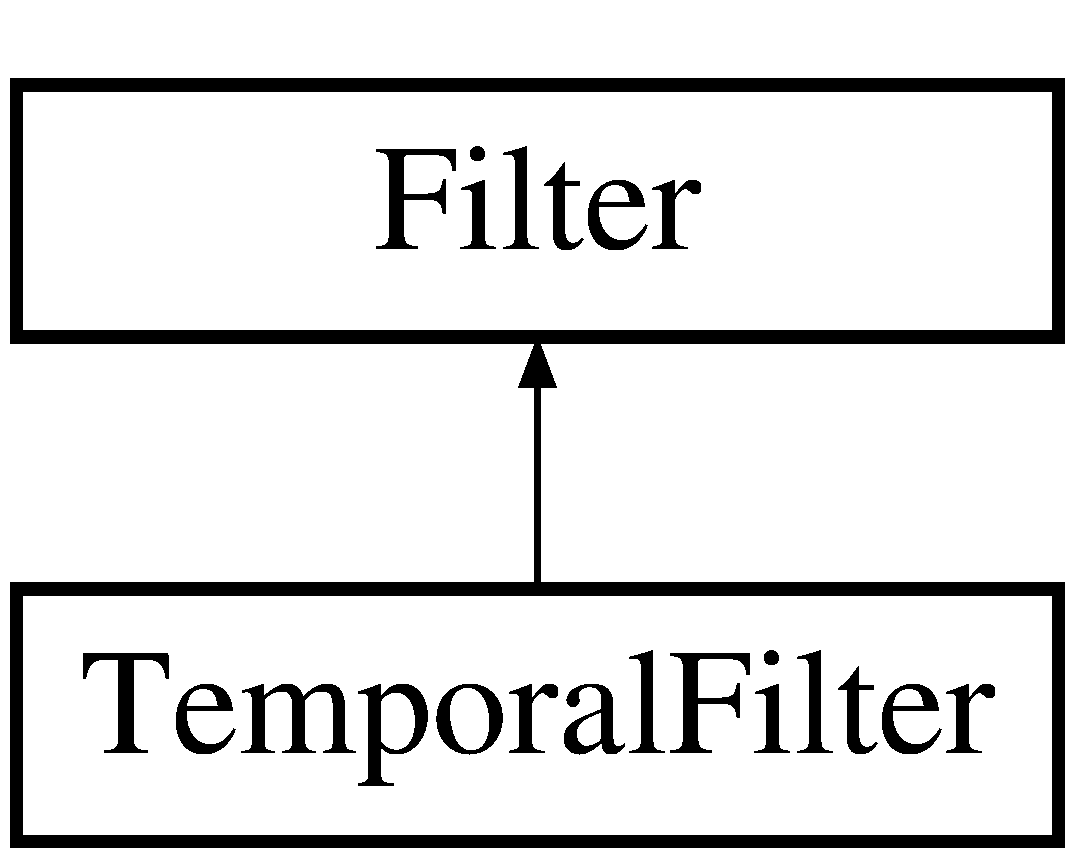
\includegraphics[height=2.000000cm]{class_temporal_filter}
\end{center}
\end{figure}
\subsection*{Public Member Functions}
\begin{DoxyCompactItemize}
\item 
\hyperlink{class_temporal_filter_a251e59cf00b8978af4bdb662573ba7f5}{Temporal\+Filter} (int d)
\item 
std\+::vector$<$ float $>$ \hyperlink{class_temporal_filter_ae08295aa926fa2bdfc64a5836cc0ac3a}{update} (std\+::vector$<$ float $>$ \&input\+Scanline)
\end{DoxyCompactItemize}


\subsection{Detailed Description}
Temporal Median filter class. 

\begin{DoxyAuthor}{Author}
Raj Singh (\href{mailto:rajvikrams@gmail.com}{\tt rajvikrams@gmail.\+com}) 
\end{DoxyAuthor}
\begin{DoxyVersion}{Version}
0.\+1 
\end{DoxyVersion}
\begin{DoxyDate}{Date}
09-\/11-\/2017
\end{DoxyDate}
Implements an \hyperlink{class_temporal_filter_ae08295aa926fa2bdfc64a5836cc0ac3a}{update()} method that stores a maximumm of last D scanlines internally and returns the median of values over the past scanlines. The class autodetects the cores on the machine and runs one thread per core. It computes the medians across multiple threads. This is obviously useful for large scanlines with a large D. For smaller values the threads introduce an overhead.

\begin{DoxyRemark}{Remarks}
Maybe in future versions multiple threads are run only for large input data and default s to a single thread for smaller scanlines. 
\end{DoxyRemark}


\subsection{Constructor \& Destructor Documentation}
\mbox{\Hypertarget{class_temporal_filter_a251e59cf00b8978af4bdb662573ba7f5}\label{class_temporal_filter_a251e59cf00b8978af4bdb662573ba7f5}} 
\index{Temporal\+Filter@{Temporal\+Filter}!Temporal\+Filter@{Temporal\+Filter}}
\index{Temporal\+Filter@{Temporal\+Filter}!Temporal\+Filter@{Temporal\+Filter}}
\subsubsection{\texorpdfstring{Temporal\+Filter()}{TemporalFilter()}}
{\footnotesize\ttfamily Temporal\+Filter\+::\+Temporal\+Filter (\begin{DoxyParamCaption}\item[{int}]{d }\end{DoxyParamCaption})\hspace{0.3cm}{\ttfamily [inline]}}

Default constructor. Takes in D as input 

\subsection{Member Function Documentation}
\mbox{\Hypertarget{class_temporal_filter_ae08295aa926fa2bdfc64a5836cc0ac3a}\label{class_temporal_filter_ae08295aa926fa2bdfc64a5836cc0ac3a}} 
\index{Temporal\+Filter@{Temporal\+Filter}!update@{update}}
\index{update@{update}!Temporal\+Filter@{Temporal\+Filter}}
\subsubsection{\texorpdfstring{update()}{update()}}
{\footnotesize\ttfamily std\+::vector$<$float$>$ Temporal\+Filter\+::update (\begin{DoxyParamCaption}\item[{std\+::vector$<$ float $>$ \&}]{input\+Scanline }\end{DoxyParamCaption})\hspace{0.3cm}{\ttfamily [inline]}, {\ttfamily [virtual]}}

Update method takes in a scanline as a vector. Calculates the median based on the past D scanlines and returns the median values in the input\+Scanline object. 

Implements \hyperlink{class_filter}{Filter}.



The documentation for this class was generated from the following file\+:\begin{DoxyCompactItemize}
\item 
temporal\+Filter.\+hpp\end{DoxyCompactItemize}

%--- End generated contents ---

% Index
\backmatter
\newpage
\phantomsection
\clearemptydoublepage
\addcontentsline{toc}{chapter}{Index}
\printindex

\end{document}
